\documentclass[conference]{IEEEtran}
\usepackage[utf8]{inputenc}
\usepackage[spanish]{babel}
\usepackage{amsmath}
\usepackage{amsfonts}
\usepackage{amssymb}
\usepackage{graphicx}
\usepackage[left=2cm,right=2cm,top=2cm,bottom=2cm]{geometry}
\usepackage{float}
\author{\IEEEauthorblockN{Paul Percca, Ivan Sipiran} 
\IEEEauthorblockA{Pontificia Universidad Católica del Perú}
\IEEEauthorblockA{Lima, Perú}
\IEEEauthorblockA{cristian.percca@pucp.edu.pe, isipiran@pucp.edu.pe}
}
\title{Identificación Automática del Comportamiento de Clientes de una Tienda Retail mediante Secuencias de Video utilizando Aprendizaje Profundo}

\begin{document}

\begin{figure}[hbtp]
\centering
\includegraphics[scale=0.8]{Figuras/reporte.png}
\end{figure}

\maketitle

\begin{abstract}
Las tiendas físicas usan múltiples técnicas para analizar el comportamiento de sus cliente, la mayoría de estas, se centra en la captura de datos en caja, al finalizar el proceso de compra; sin embargo, se pierde información valiosa sobre la estadía del client en la tienda. Por lo tanto, identificar las zonas de la tienda más concurridas por los clientes y el grado de interés de estos frente a determinados productos, es importante para los gerentes de tienda, ya que, esa información puede ayudar a crear mejores campañas de marketing y publicidad dirigida, así como optimizar el almacenamiento y la operación de la tienda . Este artículo se enfoca en brindar una solución a través del análisis de video en una tienda retail con el fin de identificar las zonas de la tienda con mayor y menor tráfico de clientes, así como identificar las zonas con mayor demanda de consumo, es decir, zonas de la tienda donde los clientes toman mayor cantidad de productos, utlizando modelos del estado del arte en deep learning como son object detection (YOLOv3) y pose estimation (HRNet).

\end{abstract}

\begin{IEEEkeywords}
Object Detection, YOLOv3, Pose Estimation, HRNet
\end{IEEEkeywords}

\section{Introducción}
Las tiendas retail, realizan una amplia variedad de actividades, muchas de las cuales pueden ser asistidas por análisis de video, como la planificación de diseños de tiendas, basadas en estadísticas de ruta de clientes, el recuento de clientes histórico e instantáneo, entradas y salidas de tiendas, colas de pago, entre otras. Cada transacción comercial y paso durante el proceso de compra, genera una gran cantidad de datos \cite{provost2013data}, que pueden ser indicadores para la toma de decisiones.

Entre esas actividades se encuentra la prevención de pérdidas y la medición del nivel de satisfacción de sus clientes. La prevención de pérdidas se clasifica en cuatro grupos primarios: pérdidas internas (trabajadores de la tienda), externas (supuestos clientes, mediante cambio de etiquetas, fraude en la devolución de productos, entre otros), proveedores y administrativas \cite{deyle2015global}.

Por otro lado, muchos clientes se sienten frustrados debido a que no encuentran su producto deseado, ya sea por haber sido colocados en góndolas inadecuadas o en zonas de la tienda que no son muy transitadas, esto generan una mala experiencia al cliente, lo cual se traduce en pérdidas de venta. Si bien se realizan estrategias comerciales y operativas para el posicionamiento de los productos, y estudios de mercado para ello, esta información no se obtiene en tiempo real y muchas veces quedan obsoletas al ser aplicadas.

Hoy en día existen varias soluciones para análisis de datos de e-commerces, sin embargo, no se tiene mucha información de lo que sucede en la tienda física, por lo tanto, esto puede resultar en un inconveniente para los administradores de tienda. Mediante el uso de análisis de video, deep learning y procesamiento de imágenes. se tiene una recopilación más activa de la información \cite{karim2018customer}, información como, cuántos clientes visitan la tienda, cuántos de las personas que entraron a la tienda compraron, cuánto tiempo permaneció una persona en la tienda, cuál fue la trayectoria de un cliente en la tienda, o cuáles son los productos donde la gente se detiene más o menos tiempo a observar, o identificar el interés mediante los gestos que muestra un cliente al estar parado frente a un producto específico. Las respuestas a estas preguntas son  información muy importante para la toma decisiones, ya que,  se puede tener una visión general y en base a esta información realizar campañas de marketing o reorganizar la ubicación de los productos de ser necesario.

Con la ayuda de Pose Estimation los gerentes de tienda pueden evaluar el nivel de interés del cliente para la mercancía, la postura del cliente, si está de pie, estirando el brazo o agachándose para tomar un producto puede revelar los hábitos del cliente, por ello en el presente proyecto se usarán las grabaciones de cámaras de vigilancia de una tienda retail, sin embargo no es un problema fácil de resolver debido a la oclusión entre las extremidades\cite{liu2018integral}.

El enfoque de este trabajo se centra identificar las zonas de la tienda con mayor y menor tráfico y así como identificar las zonas con mayor demanda de consumo utlizando técnicas del estado del arte en deep learning como son object detection (YOLOv3) tomado de \cite{redmon2018yolov3} y pose estimation (HRNet) tomado de \cite{sun2019deep} esta información va a ser mostrada en heatmaps de manera que, pueda ser de mayor provecho para los gerentes de tienda y así tomar decisiones que ayuden a la recolocación de productos con el fin de aumentar las ventas, así mismo, este análisis se podrá realizar a demanda pudiento conocer el comportamiento de los clientes cuando se requiera.

\section{Antecedentes Teóricos}

\subsection{Redes Neuronales Artificiales (ANN)}
Las redes neuronales artificiales son un paradigma de programación inspirado en la biología que permite a un algoritmo aprender a partir de un conjunto de datos observacionales \cite{nielsen2018neural}. La investigación en este campo ha tenido grandes avances, desde que McCulloch y Pitts propusieron su modelo de neurona \cite{mcculloch1943logical}. Una neurona artificial consta básicamente de un vector entradas $X$ y una matriz de pesos $W$, una función de transferencia $f$  que es el promedio ponderado de las entradas y los pesos: $ f(X) = \sum_{j} X_j W_{i,j}$ , posteriormente se  aplica una función de activación que es una transformación no lineal de la función de transferencia $g$ como una Sigmoidal, Tangente Hiberbólica, ReLU, entre otras, $ g(X) = g(\sum_{j} X_j W_{i,j})$, como se aprecia en la Figura \ref{fig:perceptron} hasta la actualidad donde se cuenta con Deep Learning.
\begin{figure}[hbtp]
\centering
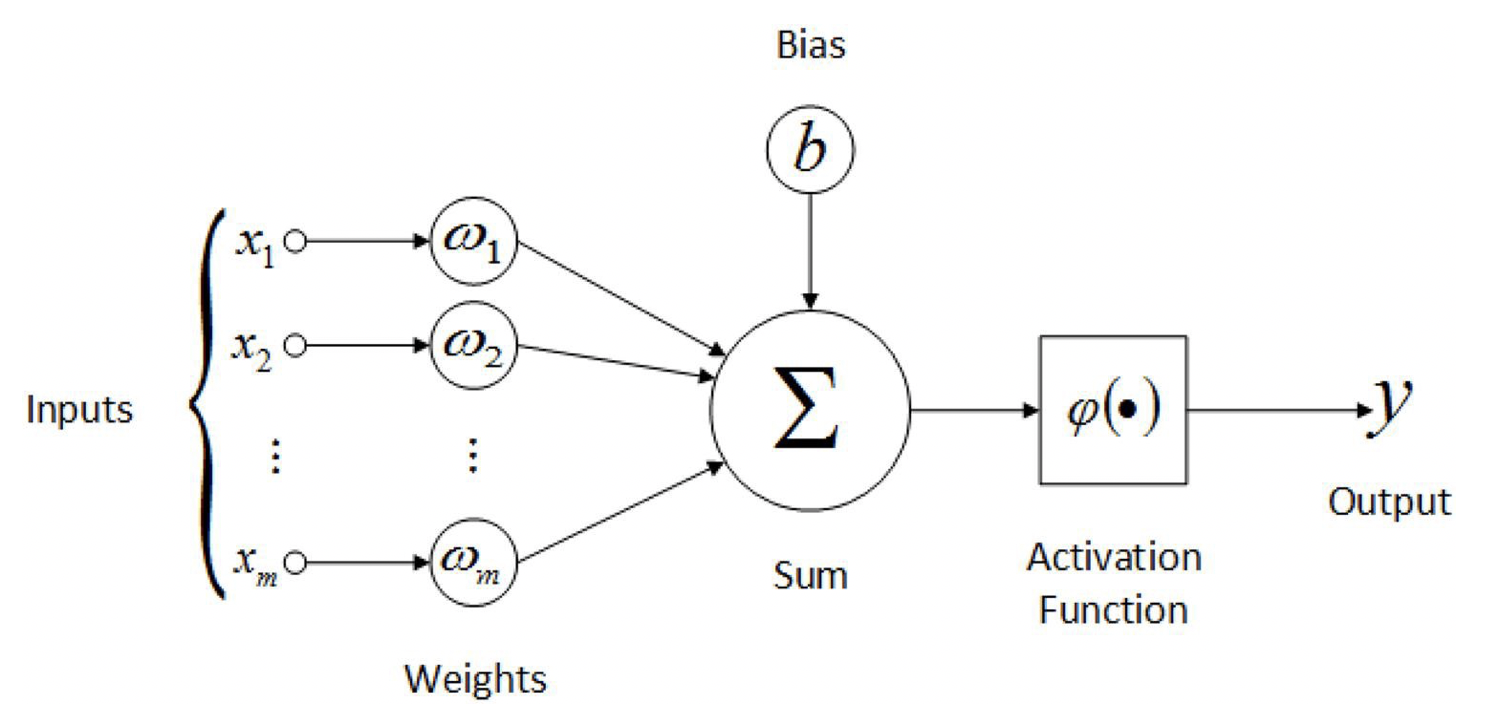
\includegraphics[width=8cm]{Figuras/perceptron.png}
\caption{Modelo de una neurona artificial}
\label{fig:perceptron}
\end{figure}

\subsection{Deep Learning}

Deep Learning permite a modelos computacionales compuestos, por multiples capas de procesamiento, aprender representaciones más complejas con múltiples niveles de abstracción, y todo esto gracias al uso de un algoritmo de backpropagation que permite ir ajustando los pesos hasta las capas anteriores \cite{lecun2015deep}, es decir, Deep Learning es un poderoso conjunto de técnicas para aprender en redes neuronales que proveen las mejores soluciones para muchos problemas en diferentes áreas como reconocimiento de imágenes, reconocimiento de voz y procesamiento de lenguaje natural \cite{nielsen2018neural}. A continuación se muestra un esquema de un modelo de Deep Learning en comparación de una Red Neuronal.

\begin{figure}[hbtp]
\centering
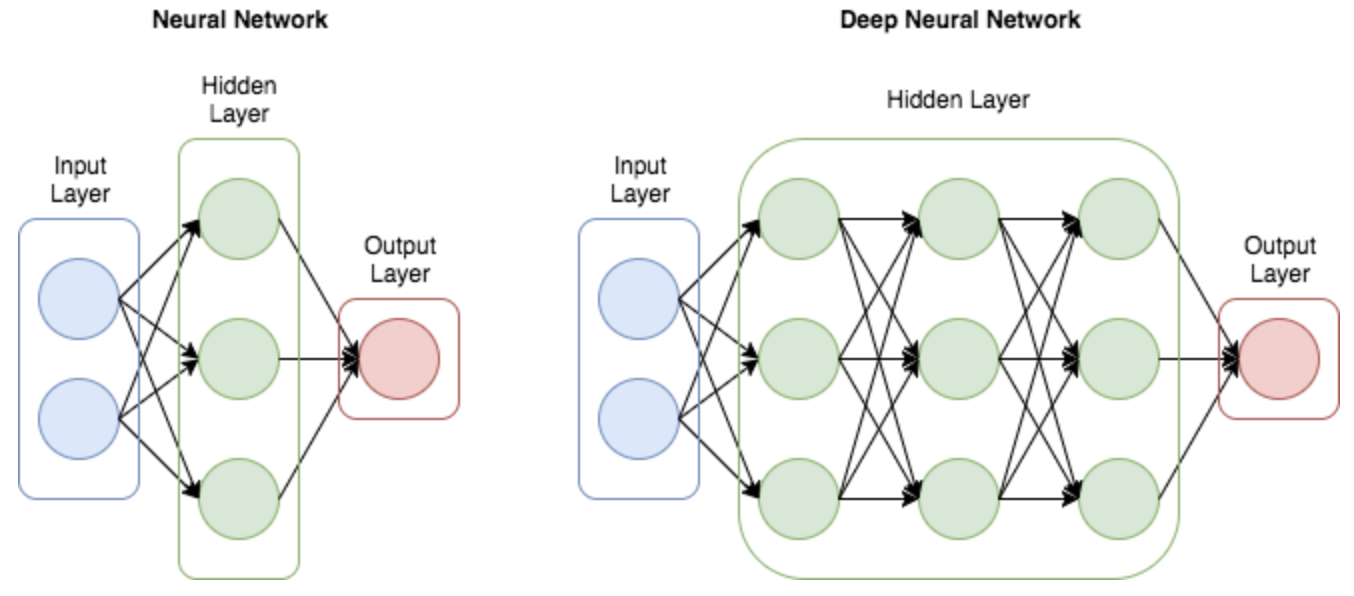
\includegraphics[width=8cm]{Figuras/deeplearning.png}
\caption{Modelo de un Red Neuronal Profunda (Deep Learning)}
\label{fig:deeplearning}
\end{figure}

\subsection{Redes Neuronales Convolucionales (CNN)}
Las Redes Neuronales Convolucionales son un tipo de redes neuronales profundas con aprendizaje supervisado usadas generalmente para procesamiento de imágenes. Las CNN contiene varias capas ocultas especializadas donde las primeras capas pueden detectar lineas, curvas y en sus capas más profundas pueden llegar a reconocer formas complejas como un rostro o la silueta de un animal.
La función lineal usada en este tipo de redes es la convolución, al convolucionar se busca obtener la relación espacial entre la imagen y los diferentes filtros o kernels que se usan, si al operar la ventana o porción de pixeles cercanos de la imagen  y el filtro se obtiene un valor alto, significa que existe una gran correlación entre la sección de imagen y dicho filtro. Por lo general se usa la función de activación ReLU, que permite suprimir la gradiente en el caso sea negativa, además de ello, es computacionalmente eficiente para este tipo de problemas. Las CNN contienen capas de Pooling cuyo objetivo es reducir la dimensionalidad de la data; como el MaxPooling donde se toma el valor máximo de la sección y se elige el valor máximo del filtro que se correlaciona con la imagen, al final del pipeline se usa capas fully connected y se le aplica una función softmax en el caso de un problema de clasificación. A continuación se muestra un ejemplo de un modelo de red Convolucional.

\begin{figure}[hbtp]
\centering
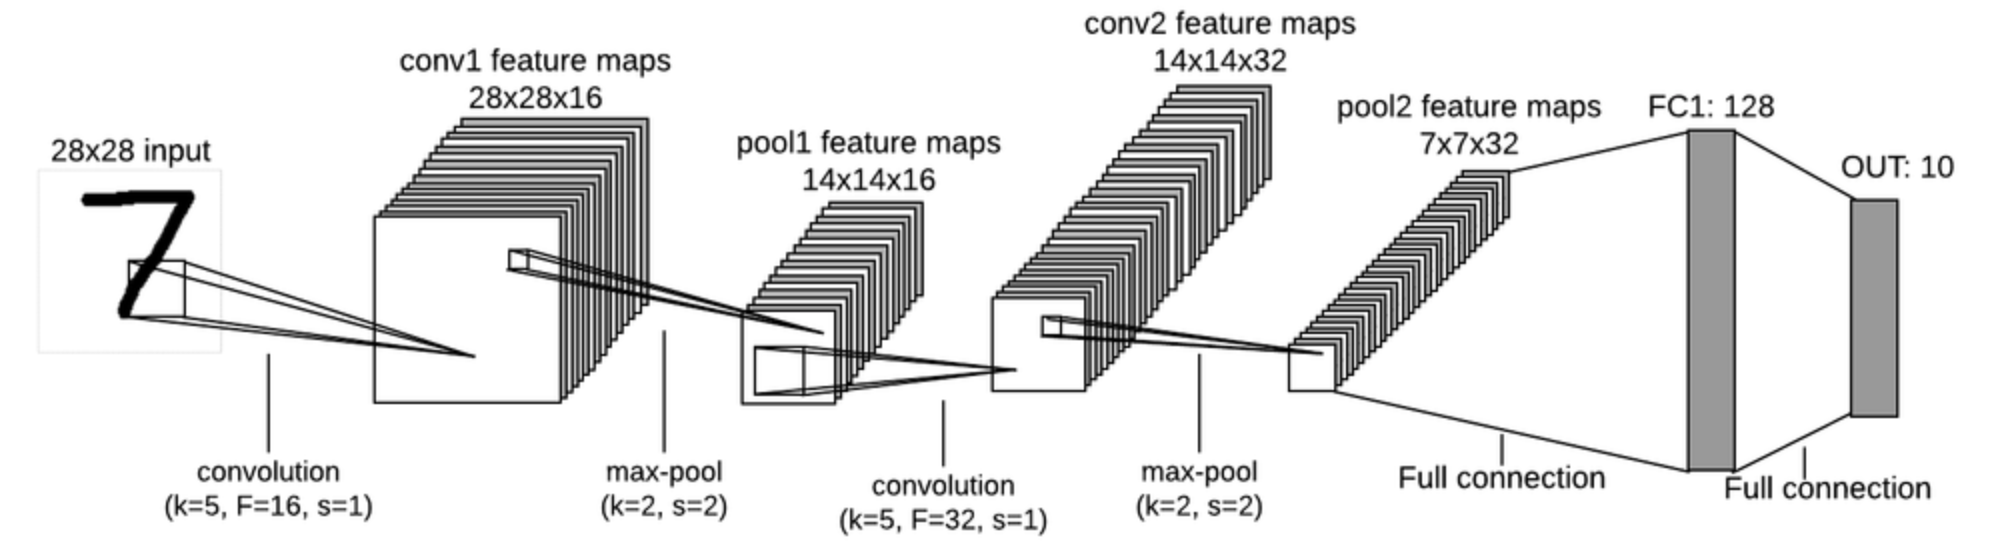
\includegraphics[width=8cm]{Figuras/cnn.png}
\caption{Modelo de una Red Neuronal Convolucional (CNN)}
\label{fig:cnn}
\end{figure}

\subsection{You Only Look Once (YOLO)}

YOLO es un modelo de Red Neuronal Convolucional usada para la detección de objetos que predice simultáneamente múltiples cuadros delimitadores y probabilidades de clase para esos cuadros, si bien YOLO comete más errores de localización, es menos probable que prediga falsos positivos, además de ello es extremadamente rápido, pudiendo correr a 45 fps en su versión base y en una versión fast a 150 fps, y esto debido a que se plantea la detección como un problema de regresión, YOLO ve la imagen completa, codifica mejor la información contextual sobre las clases y su apariencia a diferencia de otros modelos basados en propuestas de ventana deslizante y región. aprende representaciones generalizables de los objetos, al ser entrado con imágenes naturales y luego probado con ilustraciones, supera otros métodos como DPM y R-CNN \cite{redmon2018yolov3}. La arquitectura de este modelo se muestra en la Figura \ref{fig:yolo}

\begin{figure}[hbtp]
\centering
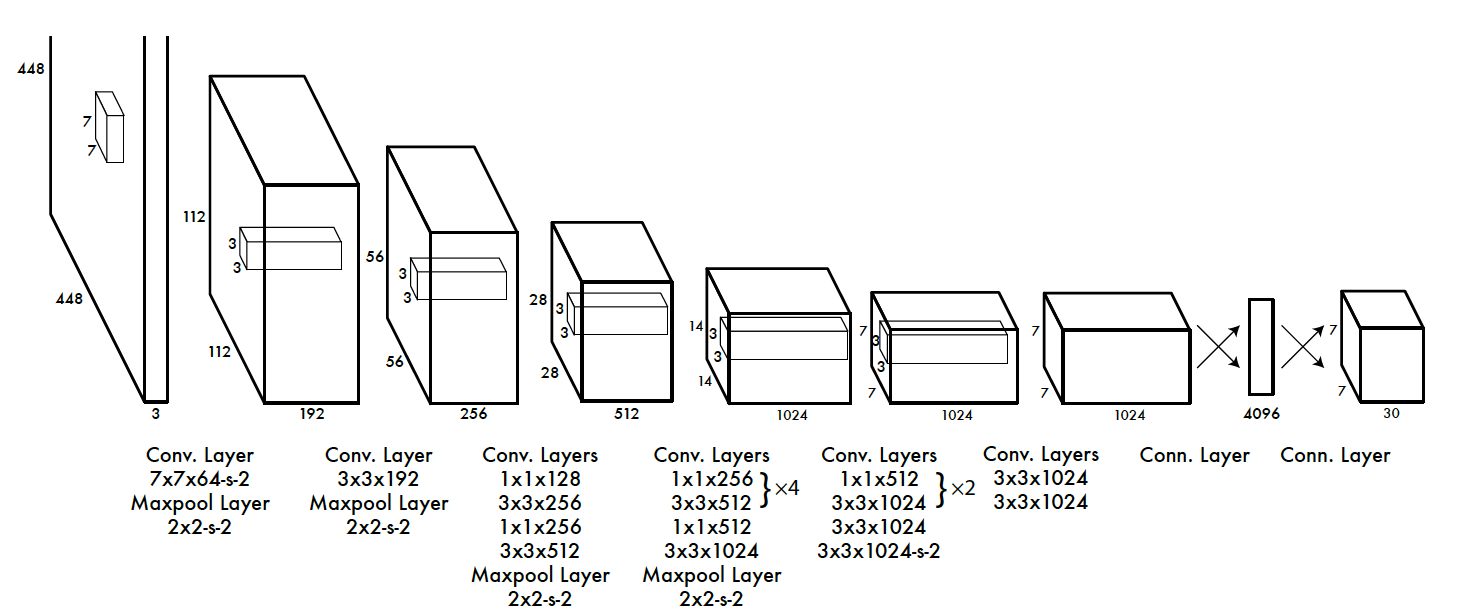
\includegraphics[width=8cm]{Figuras/yolo.png}
\caption{Arquitectura de YOLO}
\label{fig:yolo}
\end{figure}

YOLO divide cada imagen en una cuadrícula de S x S y cada cuadrícula predice B cuadros delimitadores y puntuaciones de confianza, que reflejan la confianza de que el cuadro contiene un objeto y la precisión con la que considera que el cuadro predice, de no haber una imagen en dicha celda, el puntaje es cero. Cada cuadro limitador realiza 5 predicciones x, y, w, h y el puntaje de confianza, donde (x, y) es el centro del cuadro, “w” y “h” son el ancho y el alto que se del objeto que se predice \cite{redmon2018yolov3}.


\subsection{Human Pose Estimation}
Human Pose Estimation consiste en deteminar la posición de las articulaciones humanas o keypoints, como por ejemplo codos, muñecas, rodillas, entre otras. Pose Estimation ha logrado grandes avances gracias a las CNN e incluir un regresor para determinar los heatmaps en la topología de la red neuronal, como se menciona en \cite{bulat2016human}.A continuación se muestra los 15 keypoints usados para estimar la postura humana.

\begin{figure}[hbtp]
\centering
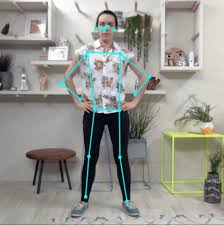
\includegraphics[width=8cm]{Figuras/poseestimation.jpeg}
\caption{Keypoints detectados con Pose Estimation}
\label{fig:poseestimation}
\end{figure}

DeePose \cite{toshev2014deeppose}, fue el primer artículo que aplicó deep learning al problema de Pose Estimation y lo formuló como un problema de regresión basado en CNN para obtener las articulaciones, además de ello se usó una cascada de regresores para mejorar las estimaciones obtenidas, este modelo usa un AlexNet como backbone, con una capa final que calcula los pares de cordenadas $(x, y)$. Las imágenes se recortan alrededor de la articulación pronosticada y se envían a la siguiente etapa, de manera que los regresores posteriores puedan ver las imágenes de mayor resolución obteniendo una mayor precisión. Posteriormente se desarrollaron otros modelos que lograron mejoras en este problema como en \cite{tompson2015efficient} , \cite{wei2016convolutional}, en \cite{carreira2016human} se utiliza un modelo de autocorrección que cambia progresivamente una solución inicial al alimentar las predicciones de error, y este proceso se denomina Retroalimentación de error iterativo (IEF), en \cite{newell2016stacked} donde la red contiene pasos de pooling y capas de upsampling apiladas, lo cual lo asemeja a un reloj , este diseño tiene por objetivo capturar la información a cualquier escala; si bien la muestra local permite identificar características pequeñas, la estimación de la pose requiere un contexto global; y en  \cite{xiao2018simple} donde se usa un modelo Resnet preentrenado con COCO dataset como backbone al cual se le agregan capas deconvolucionales al final del pipeline para estimar los heatmaps, se usa Mean Squared Error como función de pérdida. The HRNet \cite{sun2019deep} , a diferencia de los otros modelos, que iban de representaciones de alta a baja y nuevamente a alta resolución, HRNet conserva la representación en alta resolución durante todo el proces, ya que agrega gradualmente subredes de alta a baja resolución, conectando las subredes multi-resolución en paralelo, obteniendo mejores resultados. 

\section{Trabajos Relacionados}
El análisis de video en el campo de retail, es un tema relevante para los investigadores, incluso grandes  empresas han realizado investigaciones en este rubro:
\\
En \cite{ellis2002performance} se realizó una investigación en procesamiento de video en un contexto retail, basándose en un video grabado en un centro comercial, el objetivo de esta investifación era contar las personas que pasaban y saber cuántas se quedaban frente a un escaparate. De igual manera en \cite{haritaoglu2001detection} se centraron en determinar "grupos de compras" que esperaban en la cola de pago y en \cite{leykin2007detecting} utilizaron algoritmos de enjambre para agrupar clientes "grupos de compras", cabe mencionar que "grupo de compras" es un grupo de persoans que realizarían una compra conjunta, por lo tanto manejar el tráfico del grupo sería un mejor indicativo.
\\
En \cite{senior2007video} IBM planteó un sistema de vigilancia y análisis de video que se centró en la prevención de pérdidas, permitiendo al usuario elegir regiones activas y observar cuántos clientes ingresaron a una región en un período de tiempo, cuántos se detuvieron allí y cuánto tiempo pasaron estos clientes. Se muestran todas las trayectorias de los clientes y permiten al usuario "profundizar" en el video original para observar el comportamiento de los clientes seleccionados. Esta solución consistía en realizar el seguimiento de objetos genéricos y el seguimiento de caras, dicha información de apariencia, trayectoria y fotograma clave del objeto se enviaba a la base de datos, para realizar la clasificación de objetos usaron AdaBoost. Para esta investigación se usaron 6 cámaras, servidores duales Pentium de 3.6GHz para el análisis de video, administración de video y MILS. El algoritmo de seguimiento de ColourField se ejecutaba a 30 fps. La sustracción de fondo toma entre 5,5 y 8,5 ms por fotograma y el seguimiento tomaba entre 2 y 4 ms cuando había un primer plano que se debía seguir.
\\
En la detección de personas también se han realizado investigaciones como:
En \cite{gajjar2017human} donde se realiza una investación en la detección y seguimiento de humanos para videovigilancia con los datos de la Universidad Estatal de Ohio y se incorpora histogramas de gradientes orientados (HOG), la teoría de la prominencia visual y el modelo de predicción de prominencia Deep Multi-Level Network, se usó las funciones HGO para obtener una máquina de vectores de soporte (SVM) para detectar humanos en cualquier frame, para el seguimiento de personas se usó del algoritmo k - means que permitió encontrar los patrones de movimiento en los frames, lo cual es relevante para la reidentificación de la persona. además de ello se usó el algoritmo k - means para comparar y agrupar las características HOG de cuadros consecutivos para identificar el conjunto de puntos en la imagen que se asemejan a una persona en particular que se mueve en el video.
\\
En \cite{liu2018integral} se propone un Integral Pose Network (IntePoseNet) que incorpora la orientación del cuerpo y la máscara de visibilidad, la orientación del cuerpo proporciona la información global de la configuración de pose, además se fusiona con las articulares locales mediante un conjunto de capas novedosas de Orientational Message Passing (OMP) en Deep Neural Network; la máscara de visibilidad modela el estado de oclusión de cada articulación, la orientación del cuerpo es la razón principal de la auto-oclusión, en el dominio temporal, esta red incluye la información del flujo óptico y la estructura BRNN. Por lo tanto, la orientación global del cuerpo, las conexiones conjuntas locales, la información del movimiento humano, el objeto oclusivo y la consistencia temporal se consideran integralmente en la estructura de la red.

\section{Diseño de la Solución}

Para la implementación de la solución se han usado los siguientes modelos:

\subsection{Detección de Clientes}
Debido a que la detección de personas es un problema conocido se ha optado por un modelo YOLOv3 (Darknet), ya que esta arquitectura de red convolucional es extramente rápida realizando detecciones, como se explica en \cite{redmon2018yolov3}. Por ello se ha tomado un modelo preentrenado con el dataset COCO 2014, el cual se encuentra disponible públicamente en el repositorio de código fuente de ultralytics/yolov3, el cual contiene una implementación de YOLOv3 en PyTorch.

En la figura \ref{fig:yolo_salida} se observa el bounding box obtenido  al aplicar el model YOLOv3 a la imagen de un cliente.

\begin{figure}[hbtp]
\centering
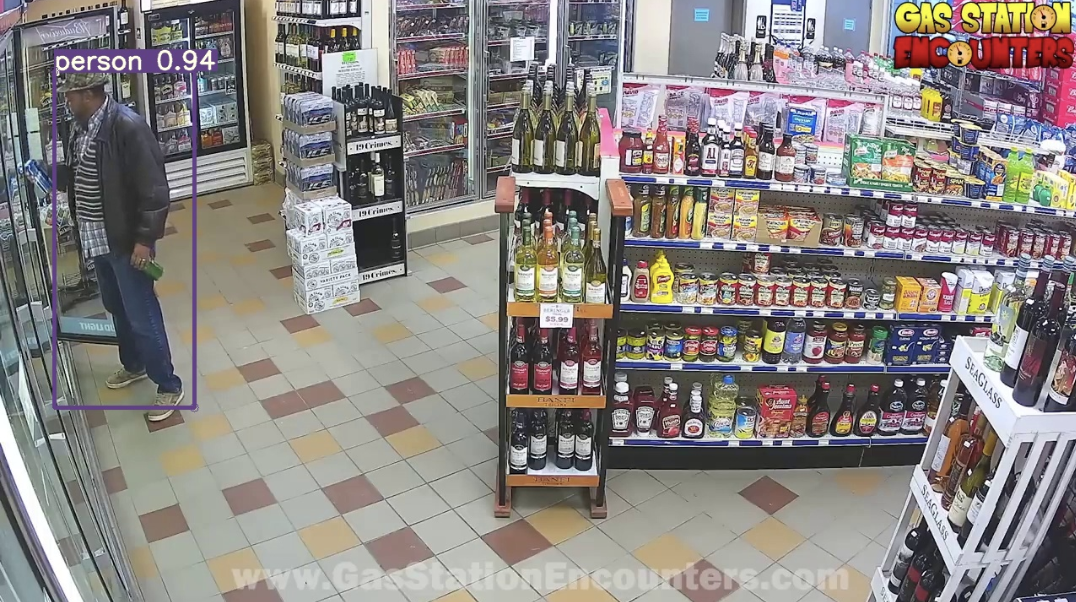
\includegraphics[width=8cm]{Figuras/yolo_salida.png}
\caption{Bounding box de un cliente en la tienda retail.}
\label{fig:yolo_salida}
\end{figure}

\subsection{Human Pose Estimation}
Para la estimación de postura humana del cliente se ha tomado el modelo HRNet \cite{sun2019deep} pre entrenado con COCO 2017, el cual es estado del arte en este campo de Pose Estimation, debido a que mantiene las representaciones de alta resolución durante todo el proceso logrando mejores resultados; con la ayuda de este modelo se obtuvo 17 keypoints (articulaciones) por cada cliente en las imágenes. Este modelo ha sido tomado del repositorio público de Github leoxiaobin/deep-high-resolution-net, el cual ha sido implementado en PyTorch.

A continuación se observa los keypoints obtenidos de dos clientes al aplicar el model HRNet a las imágenes de la tienda.

\begin{figure}[hbtp]
\centering
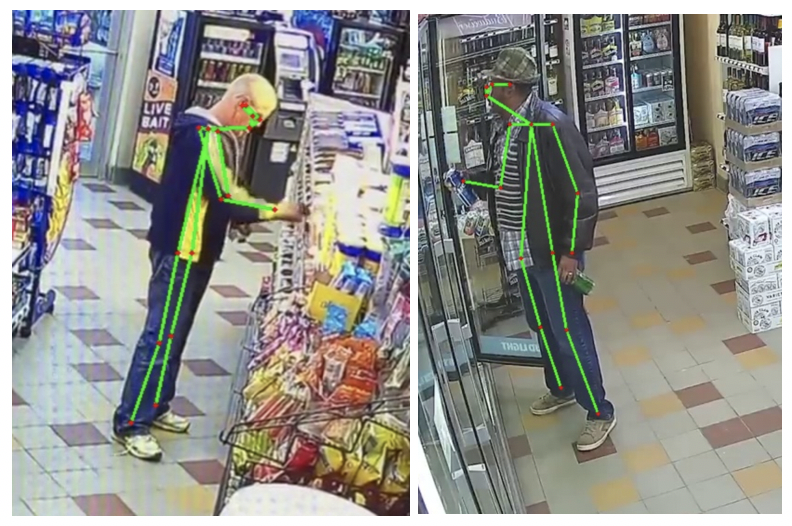
\includegraphics[width=8cm]{Figuras/pose.png}
\caption{Pose Estimation de clientes tomando productos de las góndolas.}
\label{fig:pose}
\end{figure}

\subsection{Implementación de la Solución}
A continuación se explicará de forma detallada el desarrollo de la solución presentada en este trabajo de investigación:

Debido a que se está trabajando con videos, se ha realizado las siguientes tareas:
\\
\begin{itemize}
\item Dividir el video en frames, para esto se ha usado OpenCV, partiendo de que los videos suelen tener 24, 30, o 60 frames por segundo, se ha tenido en cuenta un parámetro, el cual indica cada cuántos frames del video se guardará la imagen, es decir, por ejemplo si se tiene un video de 24 frames por segundo, y se elige como  valor del parámetro $12$, significa que se guardará solo $2$ frames por segundo del video, y esto debido a que para el problema planteado no existe mucha variación de la información de lo que ocurre de frame a frame, con lo cual se evita cálculos innecesarios, ya que de llevarse a cabo, los resultados serían muy similares de frame a frame, por ello se toma una muestra representativa.
\\
\item Detección de la posición de los clientes, para este paso se toma los frames guardados anteriormente y se procede a detectar al cliente en cada frame, aplicando el modelo YOLOv3, la salida de este modelo será un bounding box que contiene a la persona, que consta de las coordenadas de la esquina superior izquierda y las coordenadas de la esquina inferior derecha.. 
\\\\
Con estas coordenadas es posible calcular la posición $(x, y)$ del cliente, tomando como valor de $x$, la semisuma de los valores de las abscisas de las coordenadas y como $y$, el valor de la ordenada de la esquina inferior derecha, el cual muestra la parte más baja del bounding box detectado por YOLOv3, que por lo general hace referencia a los pies del cliente. Estas coordenas se guardan en una lista como se muestra  graficada en la imagen inferior donde se observa las posiciones del cliente y recorrido que este realiza a través de puntos rojos.

\begin{figure}[hbtp!]
\centering
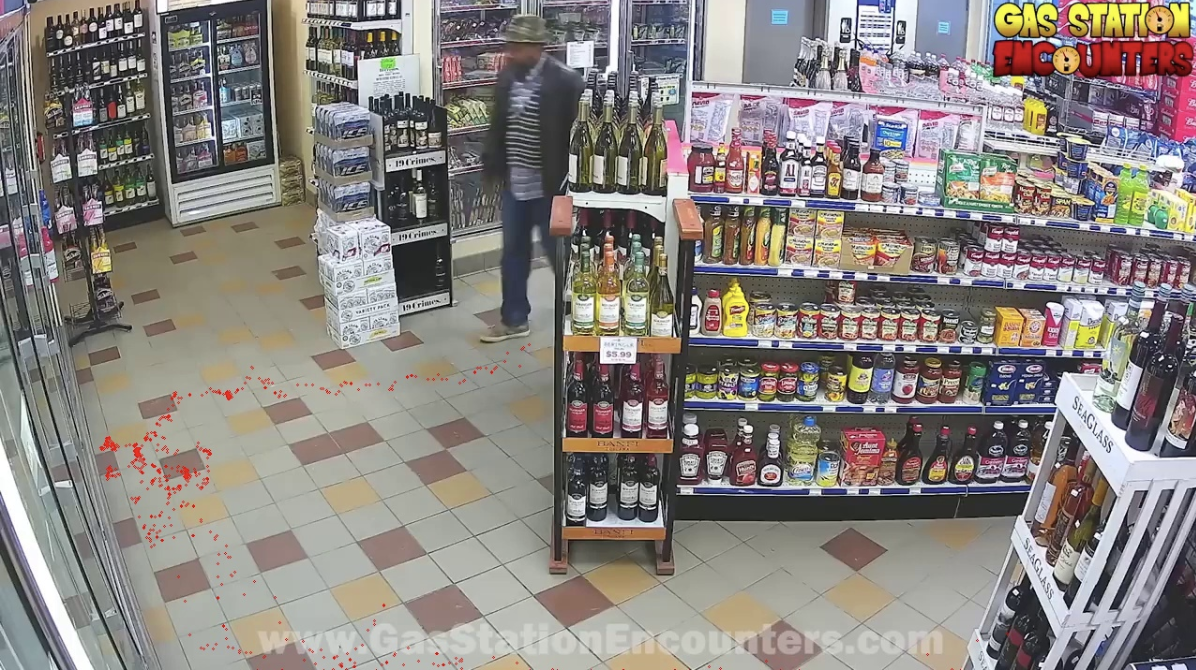
\includegraphics[width=8cm]{Figuras/recorrido.png}
\caption{Recorrido del cliente en la zona de bebidas.}
\label{fig:recorrido}
\end{figure}

Posteriormente con este listado de puntos y con la ayuda de la librería Matplotlib se ha procedido a generar un heatmap como se muestra  a continuación.

\begin{figure}[hbtp]
\centering
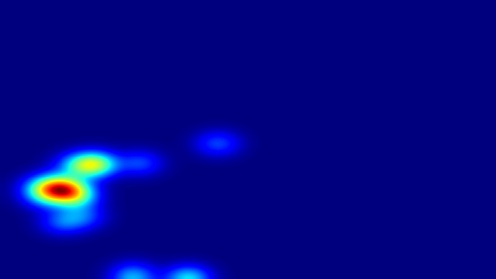
\includegraphics[width=8cm]{../Recursos/video1/video1_yolo_output_heatmap.jpg}
\caption{Heatmap de las posiciones de clientes en secuencia de video.}
\label{fig:video1_yolo_output_heatmap}
\end{figure}

En la Figura \ref{fig:video1_yolo_heatmap} se puede apreciar la salida el heatmap sobre la imagen referencial de la secuencia de videos, brindando un mejor precepción de la zona de la tienda donde el cliente ha permanecido por mayor tiempo.

\begin{figure}[hbtp]
\centering
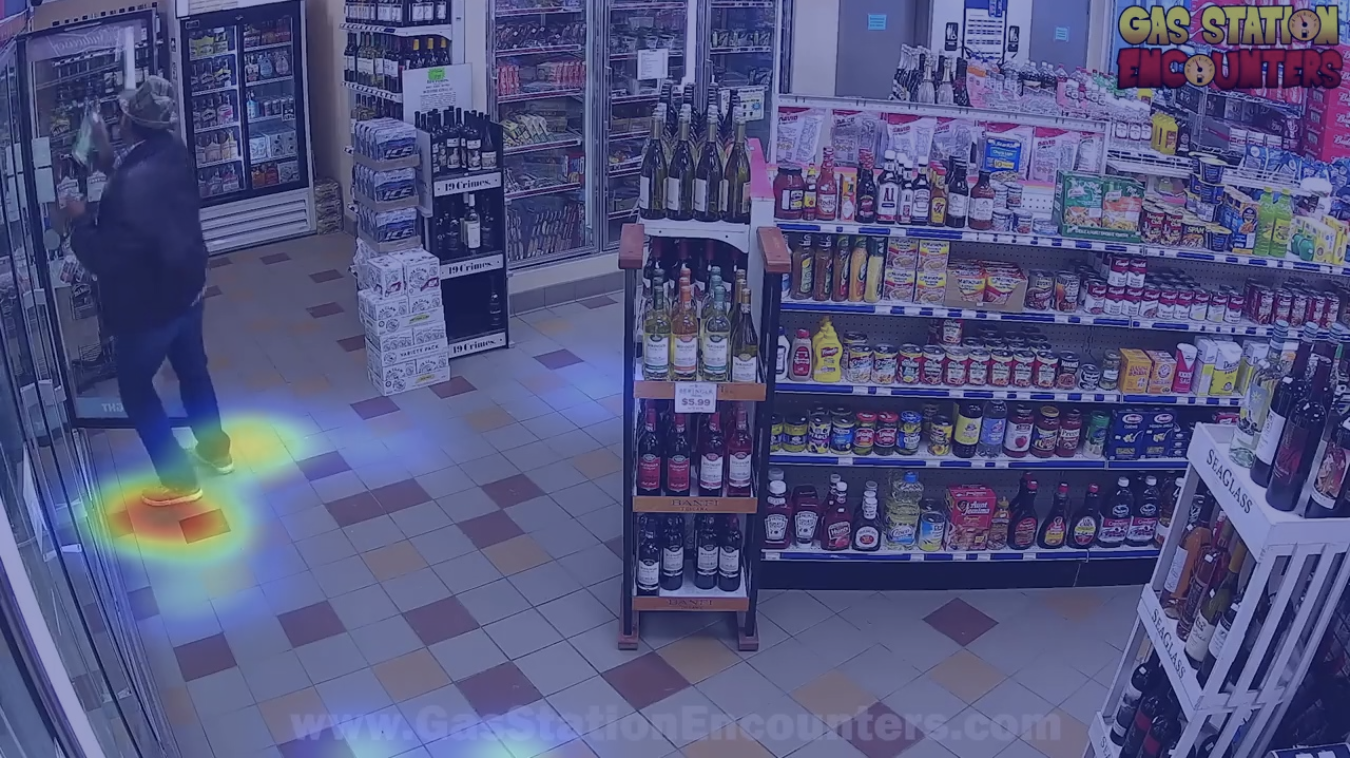
\includegraphics[width=8cm]{../Recursos/video1/video1_yolo_heatmap.png}
\caption{Heatmap de la zona donde ha habido mayor presencia del cliente en la secuencia de video.}
\label{fig:video1_yolo_heatmap}
\end{figure}

\item Preparación de imágenes para Pose detection, durante el proceso de detección de las posiciones de los clientes, al tener el bounding box como salida del modelo YOLOv3, se procedió a colocar una máscara y remover el background, de tal manera que solo se pueda visualizar el cuadro que contiene a la persona. Se ha tomado como coordenadas del cuadro la coordenada $(x, y)$ de la esquina superior izquierda y la coordenada $(x, y)$ de la esquina inferior derecha, sin embargo, se ha añadido un margen de 50px ya que si bien YOLOv3 es muy rápido, en algunas ocasiones el bounding box no es muy preciso. Este paso se ha realizado debido a que para el modelo HRNet va a ser mucho más sencillo y rápido realizar su análisis, teniendo en cuenta que la pose del cliente a detectar se encuentra en una sola zona. 
\\\\
Debido a que el modelo que usado YOLOv3 no tiene problemas en detectar múltiples personas en una misma imagen, en los frames donde existen $n$ personas a ser detectadas, se ha guardado $n$ imágenes, cada una con su máscara negra. En las siguientes imágenes se muestra cómo se ha removido el fondo cubriéndolo con una máscara negra, con excepción de la zona donde se encuentra el cliente, cabe mencionar que estas imágenes corresponden al mismo frame. \\

\begin{figure}[hbtp]
\centering
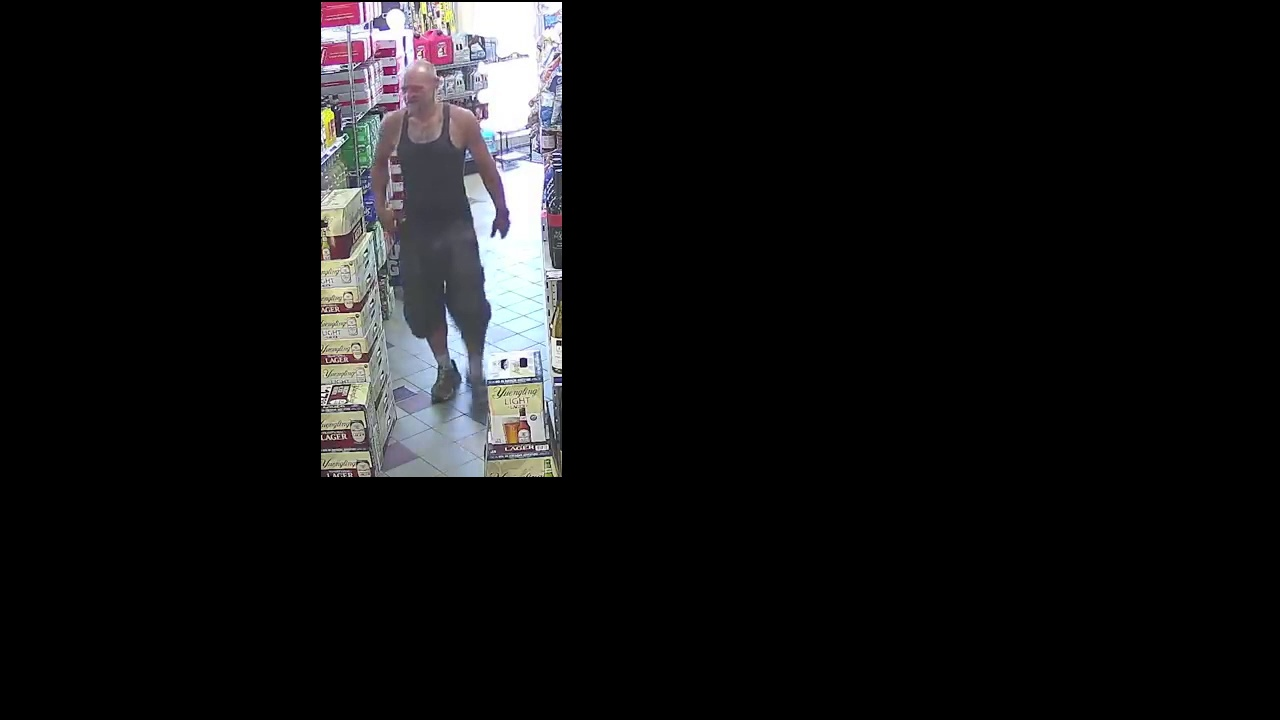
\includegraphics[width=8cm]{../Recursos/video3/frame_2_0_result.jpg}
\caption{Máscara del frame que contiene al cliente 1}
\label{fig:video3_frame_2_0_result}
\end{figure}

\begin{figure}[hbtp]
\centering
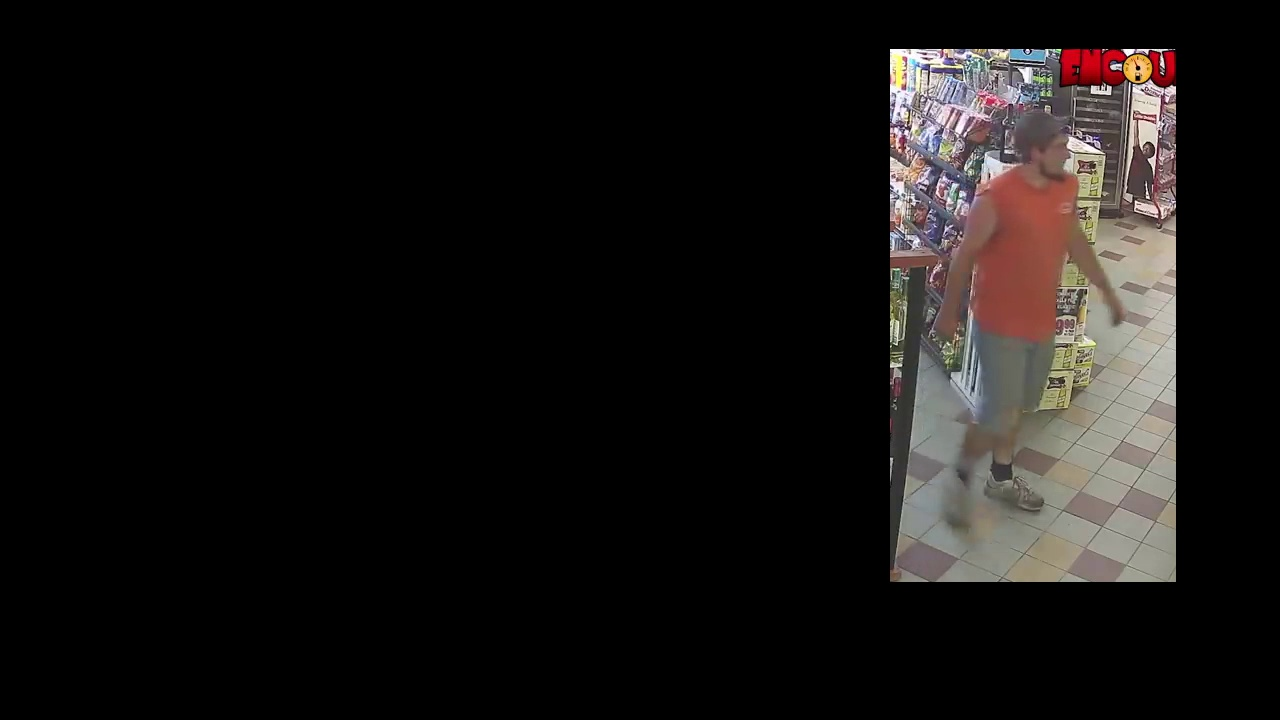
\includegraphics[width=8cm]{../Recursos/video3/frame_2_1_result.jpg}
\caption{Máscara del frame que contiene al cliente 2}
\label{fig:video3_frame_2_1_result}
\end{figure}

Esta tarea adicional se ha realizado debido a que el modelo HRNet usado, solo detecta la postura de una persona por imágen, y si en una imágen existen varias personas, la salida del modelo, no es un resultado válido.
\\
\item Detección de la posición de los clientes que están tomando un producto, para esta tarea se utilizó el modelo HRNet, con el cual se obtuvo los keypoints de las distintas articulaciones. De dichos keypoints se han usado los concernientes a los del hombro izquierdo, codo izquierdo, muñeca izquierda, así como las del hombro derecho, codo derecho y muñeca derecha, ya que, con la ayuda de estos key points se indicará si el cliente está o no tomando un producto de las góndolas, como se muestra en la Figura \ref{fig:keypoints}

\begin{figure}[hbtp]
\centering
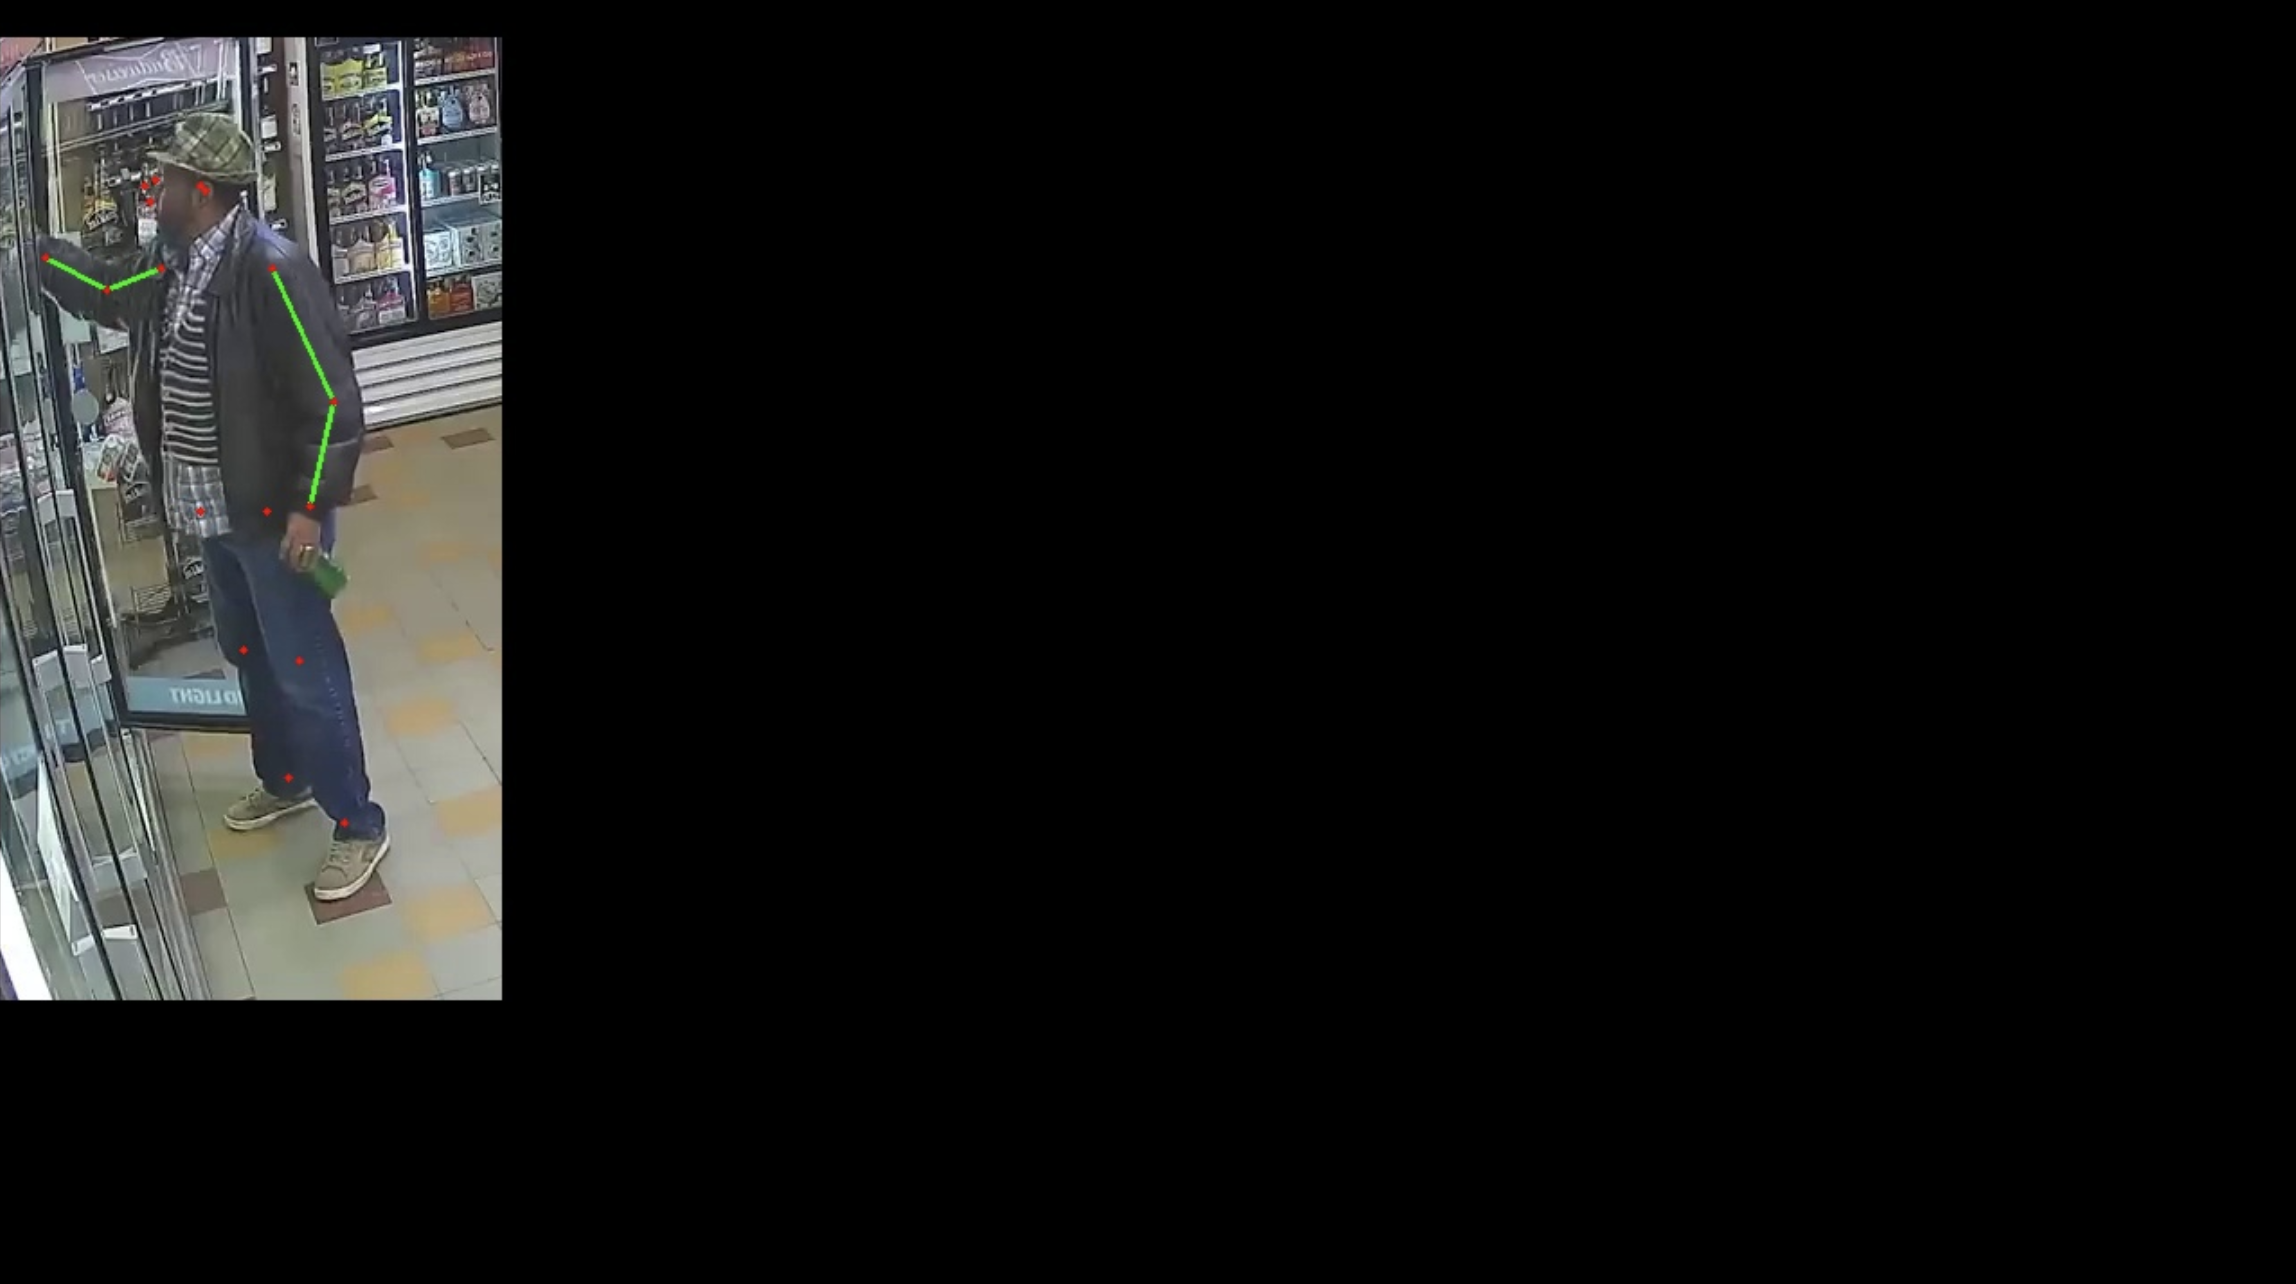
\includegraphics[width=8cm]{Figuras/keypoints.png}
\caption{Keypoints detectados con HRNet}
\label{fig:keypoints}
\end{figure}

Debido a que en ciertos frames existe oclusión de las extremidades de los clientes y en esos casos el keypoint detectado toma un valor incorrecto, que puede inclusive estar fuera del bounding box que contiene al cliente, se ha procedido a obviar dicho keypoint. 
\\
Para determinar si el cliente está tomando un producto se ha establecido un rango de ángulos que pueden formar el hombro, codo y muñeca, luego de un previo análisis se ha optado por $150º$ y $210º$, es decir si el angulo formado por esos 3 puntos es menor a  $150º$ o si es  mayor a $210º$, quiere decir que el cliente está tomando un producto, se usa dos valores, ya que el brazo del cliente puede estar hacia la derecha o hacia la izquierda, dependiendo de hacia donde esta parado el cliente, de igual manera, si la ordenada $y$ del keypoint $(x, y)$ de la muñeca es menor a la ordenada $y_1$ del keypoint $(x_1, y_1)$ del codo, lo cual quiere decir, que el cliente está contrayendo su brazo para tomar un producto.
\\\\
Luego de este tarea se ha procedido a guardar las posiciones de los clientes, de la misma forma que en los pasos anteriores, tomando en cuenta la salida del modelo YOLOv3, generando un heatmap, que indica las zonas de la tienda donde los clientes se detuvieron a tomar un producto, como se muestra en la Figura \ref{fig:video1_hrnet_output_heatmap}.  

\begin{figure}[hbtp]
\centering
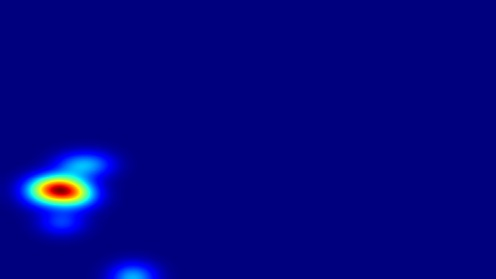
\includegraphics[width=8cm]{../Recursos/video1/video1_hrnet_output_heatmap.jpg}
\caption{Heatmap de las posiciones de clientes que toman un producto en la secuencia de video.}
\label{fig:video1_hrnet_output_heatmap}
\end{figure}

En la Figura \ref{fig:video1_hrnet_heatmap} se aprecia la zona de la tienda donde el cliente ha tomado un producto, a partir de la secuencia de video brindada.

\begin{figure}[hbtp]
\centering
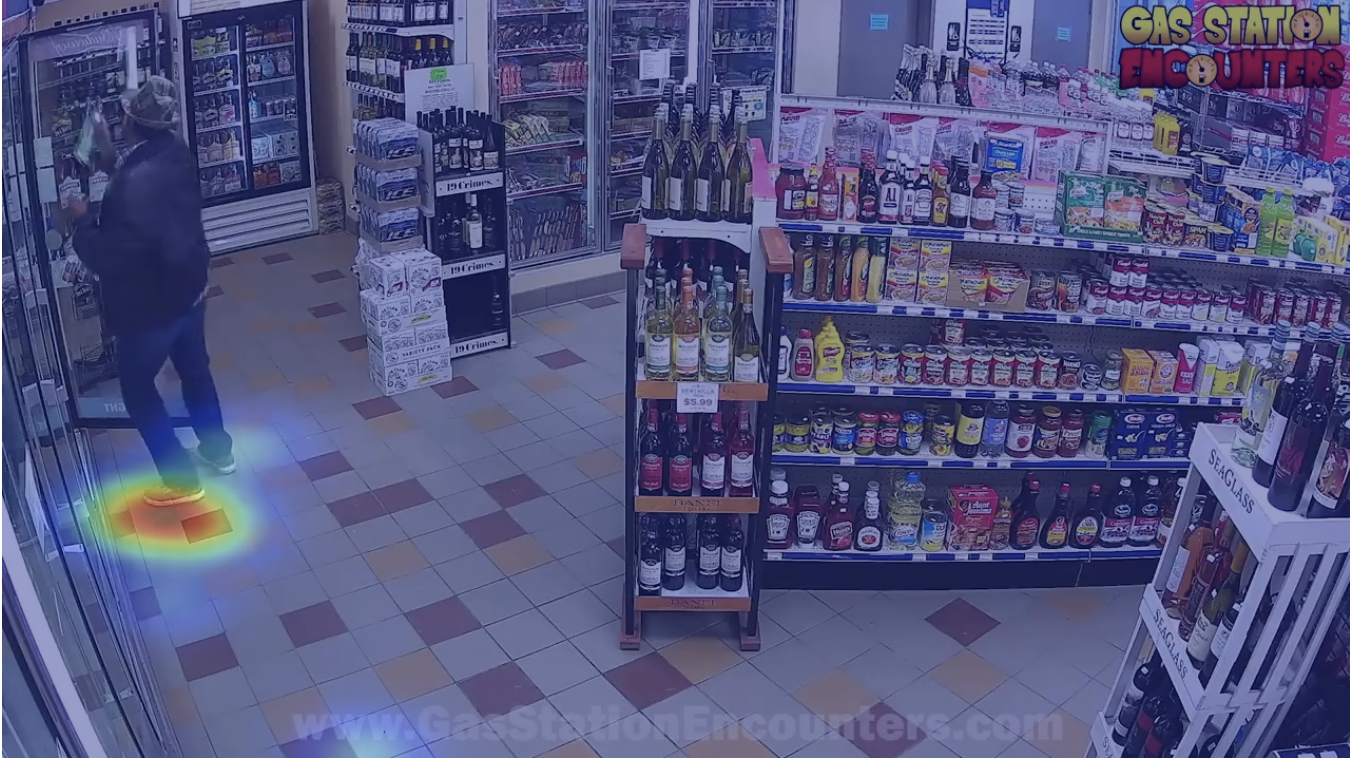
\includegraphics[width=8cm]{../Recursos/video1/video1_hrnet_heatmap.png}
\caption{Heatmap de la zona donde el cliente ha tomado productos, en la secuencia de video.}
\label{fig:video1_hrnet_heatmap}
\end{figure}

Cabe mencionar, que debido a que el heatmap de las posiciones de los clientes tomadas del modelo YOLOv3 contiene al heatmap de las posiciones de los clientes que toman un producto de las góndolas, cómputo realizado por el modelo HRNet, motivo por el cual ambos heatmaps, pueden ser muy parecidos.
\\
\item Visualización de Resultados
Para la visualización de los resultados se ha implementado una aplicación web, desarrollada en Angular, que muestra los heatmaps sobre un frame representativo de la secuencia de video, en este caso, el frame medio, para así mostrar información más valiosa del significado de los heatmaps y llegar a un mejor entendimiento de qué es lo que representan en una tienda retail, como se muestra  a continuación en la Figura \ref{fig:appweb}.

\begin{figure}[hbtp!]
\centering
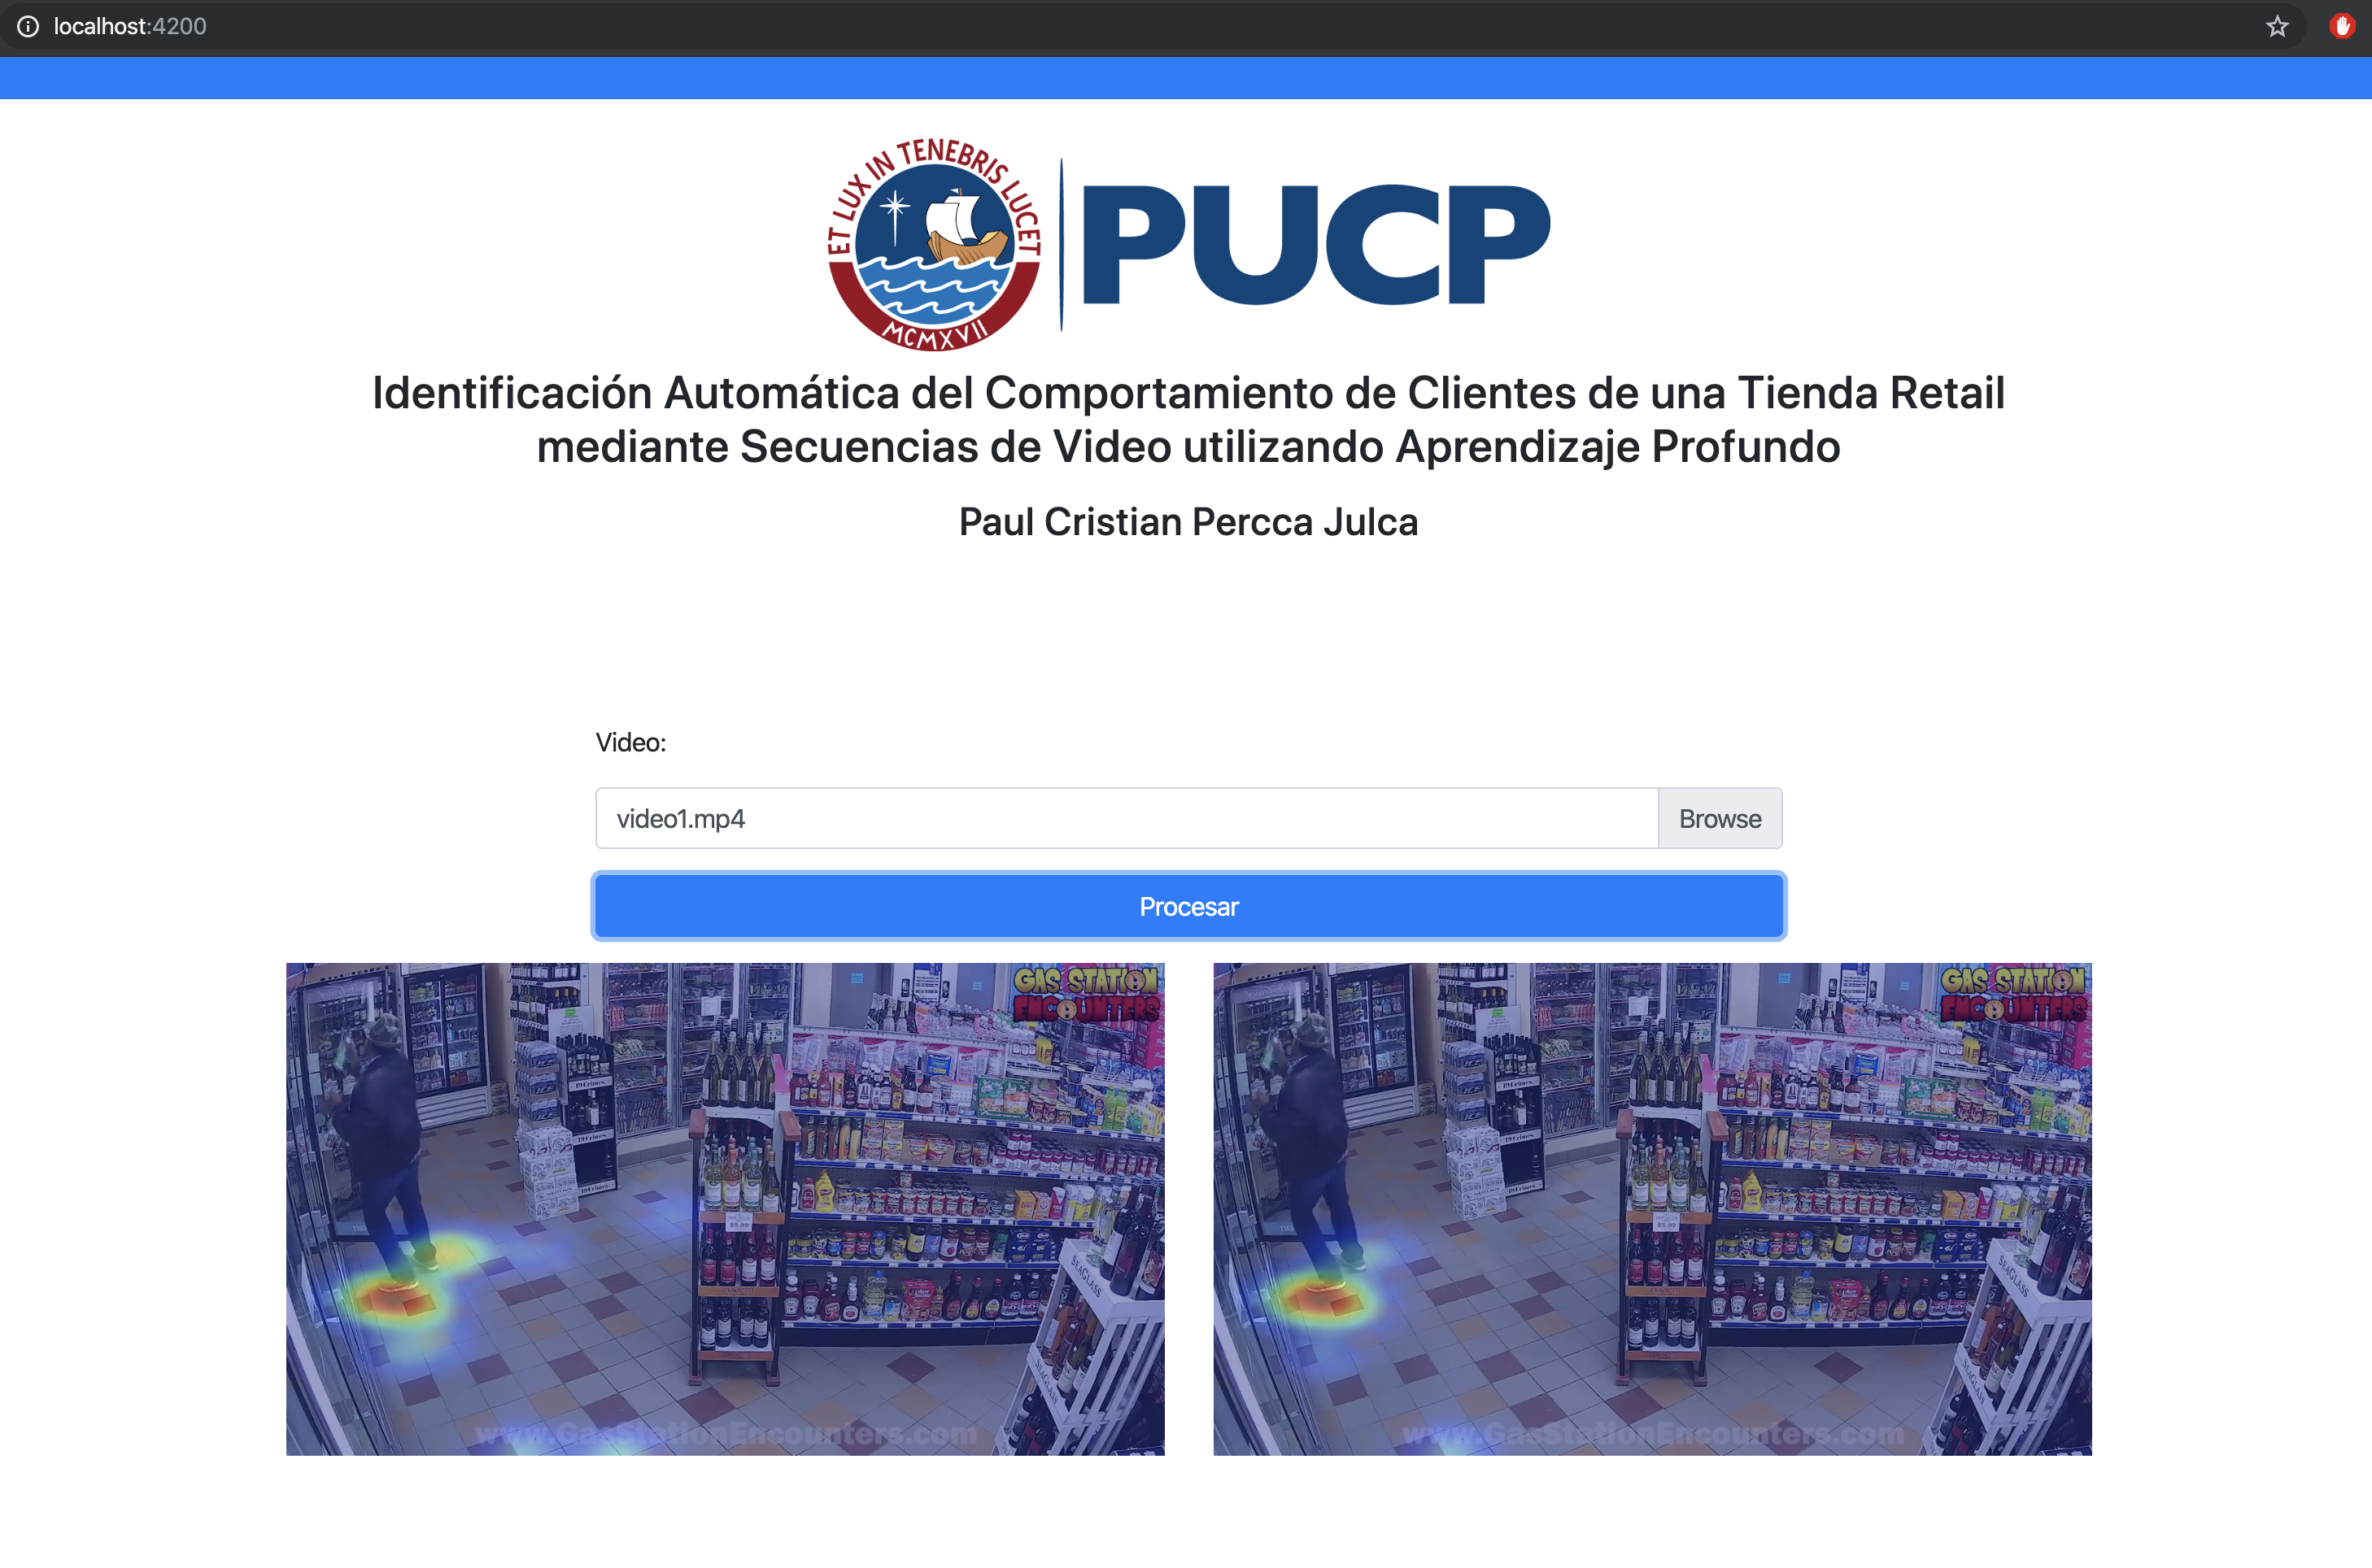
\includegraphics[width=8cm]{Figuras/appweb.png}
\caption{Aplicación web usada para subir los videos y visualizar los heatmaps.}
\label{fig:appweb}
\end{figure}
\end{itemize}

Cabe mencionar que para las pruebas de la solución planteada se han usado secuencias de video  de 720 x 1280 px de cámaras de vigilancia de la tienda de una estación de gas, tomadas de YouTube.

\section{Discusión}

Si bien ambos heatmaps pueden ser muy similares, la lectura de estos heatmaps posee un diferente significado, como se aprecia en las siguientes figuras:

\begin{figure}[hbtp]
\centering
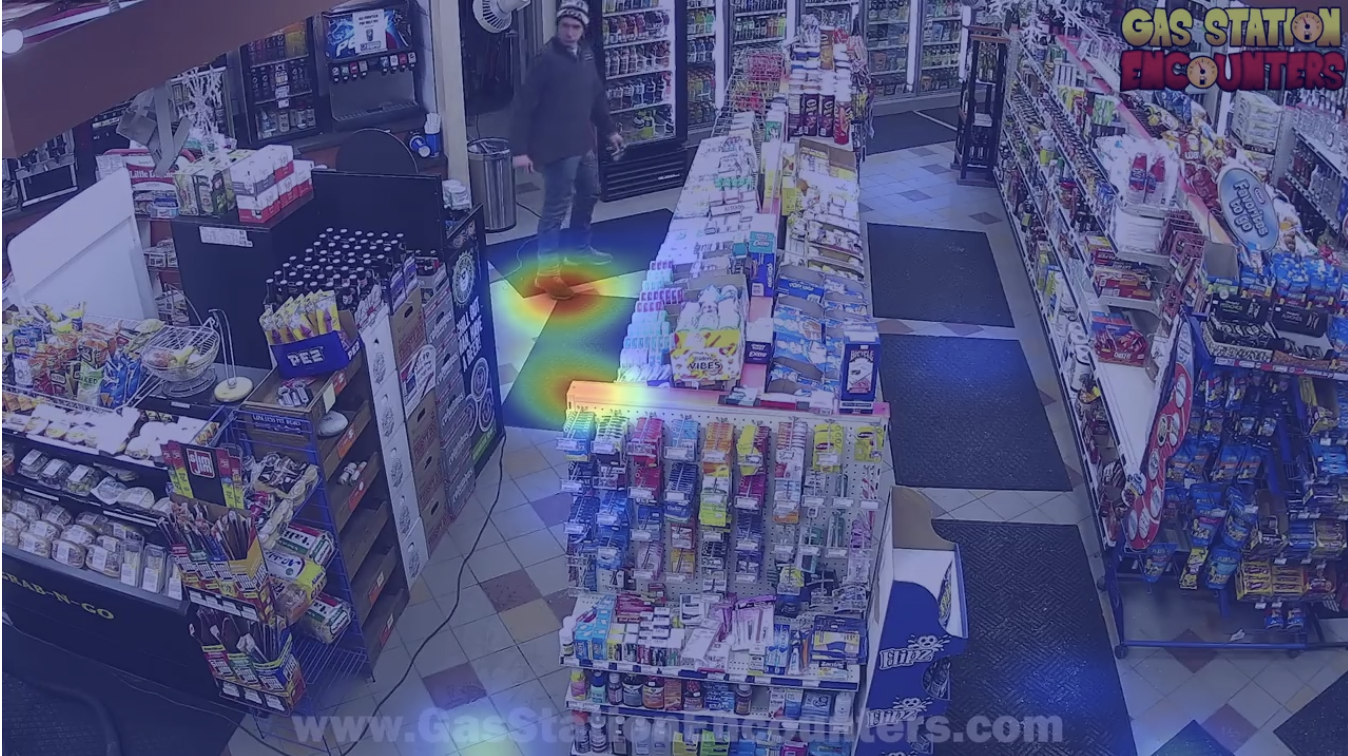
\includegraphics[width=8cm]{../Recursos/video4/video4_yolo_heatmap.png}
\caption{Heatmap de la zona donde ha habido mayor presencia del cliente en la secuencia de video.}
\label{fig:video4_yolo_heatmap}
\end{figure}

\begin{figure}[hbtp]
\centering
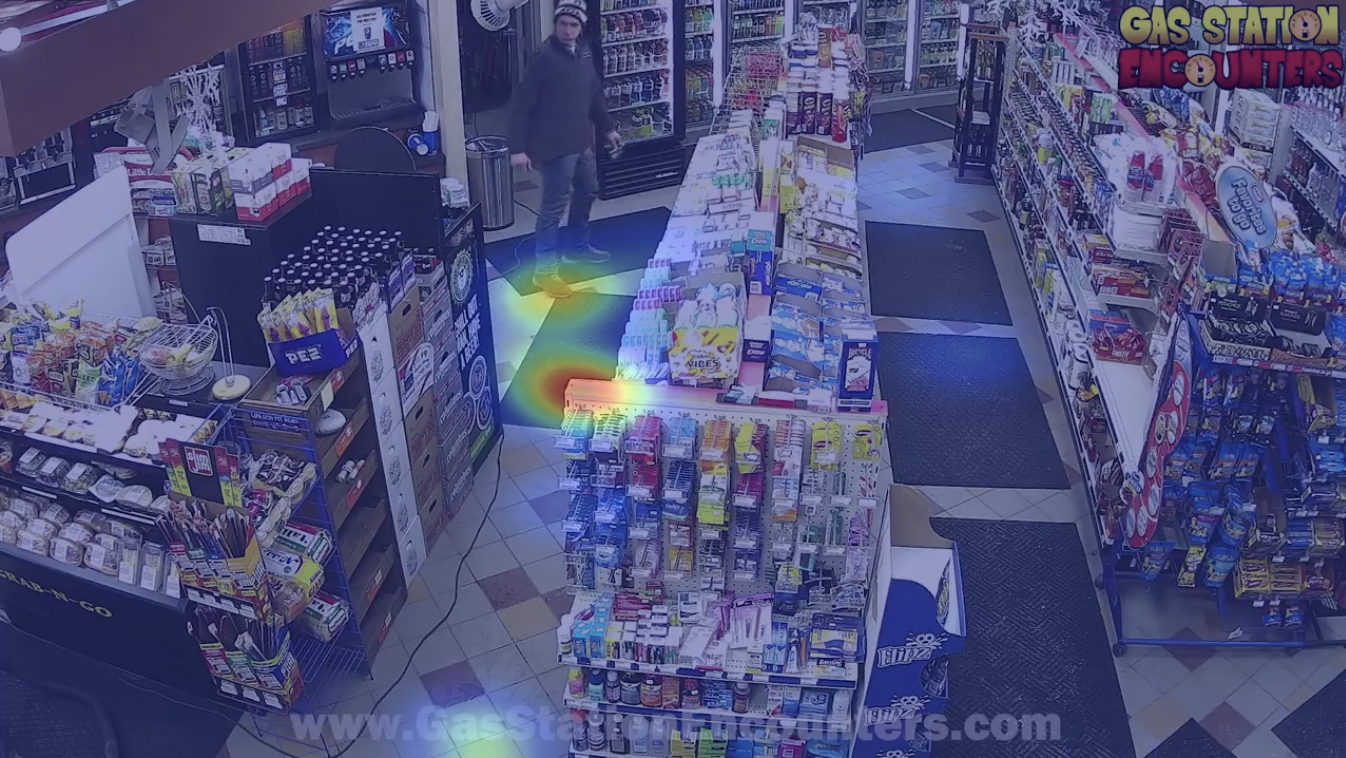
\includegraphics[width=8cm]{../Recursos/video4/video4_hrnet_heatmap.png}
\caption{Heatmap de la zona donde el cliente ha tomado productos, en la secuencia de video.}
\label{fig:video4_hrnet_heatmap}
\end{figure}


Como se aprecia en la figura \cite{fig:video4_yolo_heatmap}, el cliente ha permanecido un mayor tiempo en la zona superior, esto debido a que existe una mayor concentración de puntos en dicha zona de la imagen, en contraste con la figura \cite{fig:video4_hrnet_heatmap}, el cual muestra una mayor concetración en un una zona de calor contigua a la anterior, esto indica que el cliente ha tomado un producto en dicha zona, lo cual guarda relación con lo que ocurre realmente en el video, si bien dichos heatmaps pueden ser muy similares, ambos poseen un significado diferente.


\section{Entorno de Implementación}
La implementación fue realizada durante una etapa inicial en Google Colab con Python 3 como entorno de desarrollo, un GPU como acelerador de hardware, además de ello se usó  la biblioteca de Redes Neuronales, PyTorch en su versión 1.2. Para el manejo de vectores y matrices, se usó la extensión Numpy, se utilizó la librería Pandas, de igual manera, para el tratamiento de las imágenes se usó OpenCv versión 4.1 y Matplotlib versión 3.1 para la generación de los heatmaps.

Durante el desarrollo de la herramienta de visualización de los heatmaps se usó una  aplicación web Angular en su versión 6 con la librería de componentes ng-bootsrap 2.0 y para los estilos de la aplicación se usó Bootstrap 4.

Para la parte backend, se usó una aplicación server Api Rest implementada en Flask en la versión 1.1

\section{Conclusiones y Trabajos Futuros}

En base la implementación realizada, se ha identificado que es posible desarrollar soluciones software para la industria retail, teniendo como base modelos de visión computacional, como lo son YOLOv3 para detección de objetos y HRNet para la detección de la postura humana, con los cuales se puede brindar indicadores que ayuden a la toma de decisiones a las tiendas retail, con el fin de tener una mejor perspectiva del tránsito en las tiendas y zonas más visitadas de las mismas.

Como trabajos futuros, se plantea generar más indicadores con información relevante para la toma de decisiones, así como la implementación de otros modelos de redes neuronales convolucioanles, cuyo foco sea la seguridad y la detección de fraudes.

\bibliographystyle{plain}
\bibliography{Bibliografia}

\end{document}


%\begin{figure}[hbtp]
%\centering
%\includegraphics[scale=0.8]{Figuras/reporte.png}
%\end{figure}
